%%******************************************************************************
%%
%% nomenclatura.tex
%%
%%******************************************************************************
%%
%% Title......: Nomenclatura
%%
%% Author.....: GSCAR-DFKI
%%
%% Started....: Nov 2013
%%
%% Emails.....: renan028@gmail.com
%%
%% Address....: Universidade Federal do Rio de Janeiro
%%              Caixa Postal 68.504, CEP: 21.945-970
%%              Rio de Janeiro, RJ - Brasil.
%%
%%******************************************************************************


%%******************************************************************************
%% CHAPTER - Nomenclatura
%%******************************************************************************
\section{Nomenclatura}
\begin{itemize}

\item \emph{Stoplog}: Bloco de a�o com vinte metros de comprimento, tr�s metros
de altura e tr�s metros de largura (20x3x3 m). O fluxo de �gua do rio �
controlado pelo empilhamento de \emph{Stoplogs} (figura~\ref{nomenclatura_1} ).


\item \emph{Lifting Beam}: Estrutura mec�nica respons�vel pelo deslocamento de
\emph{Stoplogs}, composta por: duas garras n�o atuadas, duas chaves de opera��o, vigas e mecanismo. Um guindaste atua neste mecanismo (figura~\ref{nomenclatura_2}).
    
\item \emph{Guindaste}: O guindaste � capaz de sustentar todo o conjunto
\emph{Lifting Beam}/\emph{Stoplog} e � atuado por um motor el�trico
(figura~\ref{nomenclatura_3} ).

\item \emph{Garra pescadora}: Garra localizada no \emph{Lifting Beam} que se
prende ao \emph{Stoplog}. O mecanismo � composto por duas garras (figura~\ref{nomenclatura_4} ).

\item \emph{Chave de opera��o}: Localizada na viga principal, pr�xima � garra
pescadora, seleciona o modo de opera��o.  Atuada manualmente (figura~\ref{nomenclatura_5} ).

\end{itemize}

\begin{figure}[H]
    \centering
    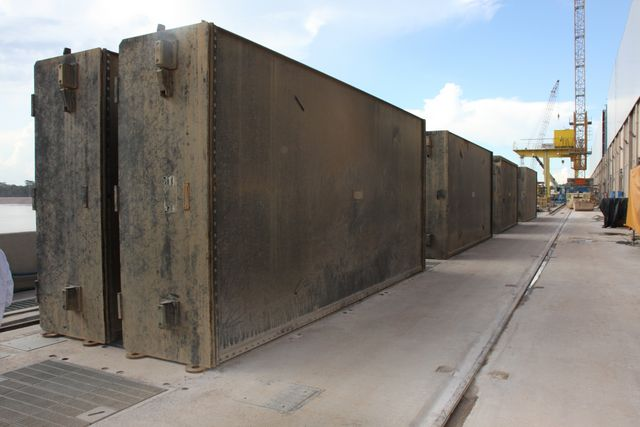
\includegraphics[width=1\columnwidth]{figs/nomenclatura/1.jpg}
    \caption{Stoplogs.}
    \label{nomenclatura_1}
\end{figure}

\begin{figure}[H]
    \centering
    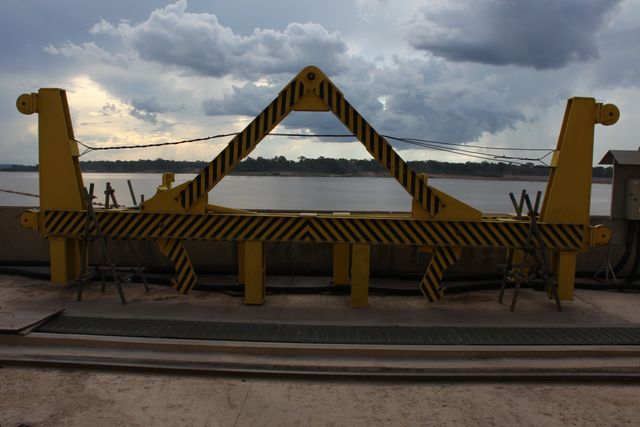
\includegraphics[width=1\columnwidth]{figs/nomenclatura/2.jpg}
    \caption{\emph{Lifting Beam}.}
    \label{nomenclatura_2}
\end{figure}

\begin{figure}[H]
    \centering
    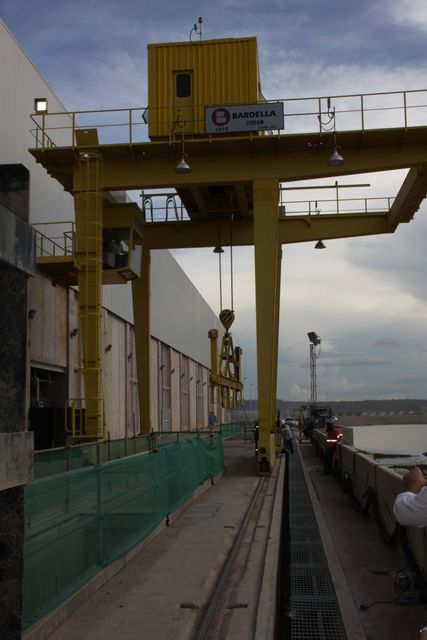
\includegraphics[width=1\columnwidth]{figs/nomenclatura/3.jpg}
    \caption{\emph{Guindaste}.}
    \label{nomenclatura_3}
\end{figure}

\begin{figure}[H]
    \centering
    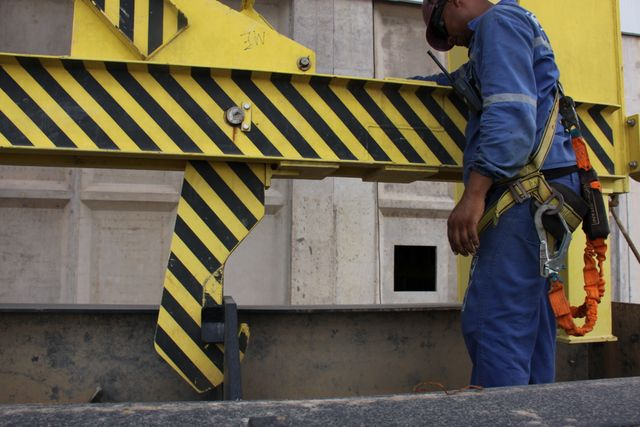
\includegraphics[width=1\columnwidth]{figs/nomenclatura/4.jpg}
    \caption{\emph{Garra pescadora}.}
    \label{nomenclatura_4}
\end{figure}

\begin{figure}[H]
    \centering
    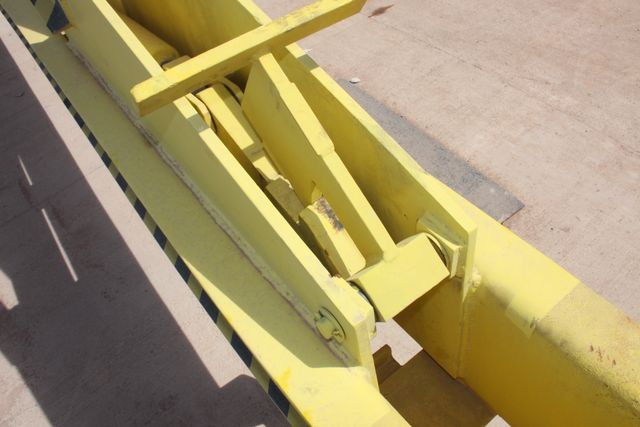
\includegraphics[width=1\columnwidth]{figs/nomenclatura/5.jpg}
    \caption{\emph{Chave de opera��o}.}
    \label{nomenclatura_5}
\end{figure}
